\documentclass[conference]{IEEEtran}
\IEEEoverridecommandlockouts
% The preceding line is only needed to identify funding in the first footnote. If that is unneeded, please comment it out.
\usepackage{cite}
\usepackage{amsmath,amssymb,amsfonts}
\usepackage{algorithmic}
\usepackage{graphicx}
\usepackage{textcomp}
\usepackage{xcolor}

\def\BibTeX{{\rm B\kern-.05em{\sc i\kern-.025em b}\kern-.08em
    T\kern-.1667em\lower.7ex\hbox{E}\kern-.125emX}}
\begin{document}

\title{A Scallable Microarchitecture for an \\ eBPF-based Packet Filter Accelerator\\
{\large Project Proposal}
}

\author{\IEEEauthorblockN{Jefferson Cavalcante}
\IEEEauthorblockA{\textit{MDCC} \\
\textit{Universidade Federal do Ceará}\\
Fortaleza, Brazil \\
jeff.cav@alu.ufc.br}
}

\maketitle

\begin{abstract}
TODO
\end{abstract}

\begin{IEEEkeywords}
component, formatting, style, styling, insert
\end{IEEEkeywords}

\section{Introduction}
Nowadays' Data Centers servers are able to leverage thousands of client applications with the use of containers, a lightweight Operating-System-level virtualization technique \cite{fouladi:2019:laptop2lambda}. In such a scenario, it is ideal that the expensive CPU cores on Data Centers servers spend most of their time running client applications to maximize revenue, also avoid having idle cores that lead to expensive resource underutilization \cite{li:2020:dccpi}. 

However, having non-underutilized cores doesn't necessarily mean higher revenue per core. For example, in \cite{emmerich:2018:ovs-throughput} authors show how virtual network switching can increase CPU load, also reduce throughput and introduce latency and jitter to virtual networks, impacting applications performance and reducing revenue per core of the data center, although such expensive cores are busy but not processing paying-clients' applications.

Developers from Suse presented in 2020, at the FOSDEM conference, how one of the most used tools for containers orchestration, Kubernetes, make heavy use of Linux netfilter engine for load balancing and firewalling, which in turn leads to prohibitive numbers in terms of rules load and processing time required for packet filtering as the number of applications increases to dozens of thousands \cite{restecki:2020:iptables-ebpf}.

For scenarios in which there's the need for high number of packet filtering rules, extended Berckeley Packet Filter (eBPF) programs are a viable solution. These programs can be responsible for packet processing and filtering in a very efficient way when compared to how the Linux kernel does the same with netfilter \cite{vieira:2020:fast-ebpf-xdp} \cite{miano:2018:ebpf-experience} \cite{bertrone:2018:ebpf-throughput}, as illustrated in Figure-\ref{fig:ebpf-throughput}.

\begin{figure}[ht]
    \centering
    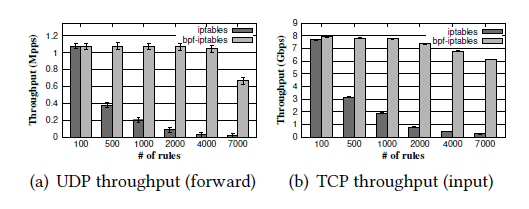
\includegraphics[width=0.45\textwidth]{figures/ebpf.png}
    \caption{ Throughput with iptables and eBPF-based packet filtering in Linux kernel \cite{bertrone:2018:ebpf-throughput}.}
    \label{fig:ebpf-throughput}
\end{figure}

Although more efficient, at higher data rates this solution still overloads expensive server cores with packet filtering programs for load balancing, firewalling and intrusion detection for example, which are non-paying-clients applications and reduces data center revenue per core. To address this problem, Netronome built support for offloading eBPF programs to cheaper cores in their smartNICs, and presented a tutorial on the prestigious SIGCOMM conference in 2018 on how to leverage their solution to offload a load balancer written in eBPF \cite{beckett:2018:ebpf-xdp}. At the time, their solution was still limited and not scallable for multiple eBPF programs and did not integrate with their Single-Root I/O Virtualization (SR-IOV) solution, a technology that allows hardware virtualization of PCIe devices and is widely used by network cards to virtualize network interfaces for exclusive use by virtual machines and containers.

\section{Problem Statement}
To support the needs of modern Data Centers workloads and maximize their revenue per CPU core, one of the problems to be addressed is the minimization of packet filter processing on these cores by offloading this task to purpose-specific hardware in a scallable and efficient way.

\section{Related Work}
\label{sec:rel-works}

In recent years, a series of works on purpose-specific hardware to increase energy or time efficiency of specific tasks has emerged, achieving exciting results when compared to when such tasks run on general purpose CPUs. For example, in 2016 a computer architecture which organizes processing units into tiles with near memory for faster neural network processing, the ISAAC \cite{shafiee2016isaac} architecture was proposed to bring together near memory processing and a memristor-based dot product engine, which allows high energy efficiency in matrix-vector multiplications by performing then in the analog domain, as shown in Figure-\ref{fig:isaac}. More recently, in 2019, ISAAC was evolved into PUMA, with more complex purpose-specific cores (processing units) and tiles, an Instruction Set Architecture (ISA) and a compiler to convert high-level Deep Neural Networks implementation into the PUMA ISA, bringing programmability and generality for execution of a wide range of neural network architectures \cite{ankit2019puma}.

\begin{figure}[ht]
    \centering
    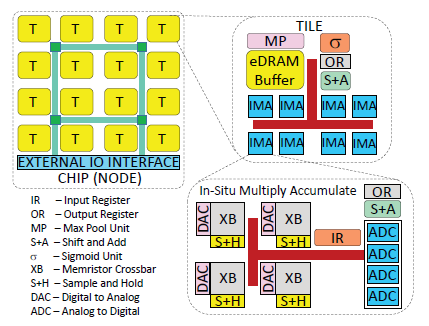
\includegraphics[width=0.4\textwidth]{figures/isaac.png}
    \caption{Tiled ISAAC architecture for processing of convolutional neural networks \cite{shafiee2016isaac}.}
    \label{fig:isaac}
\end{figure}

Likewise, recent advances in the development of smartNICs brought the possibility of offloading part of eBPF processing required by modern data center workloads, although current solutions are still very limited and prevent Data Centers from benefiting from their packet filter offloading capabilities \cite{miano:2019:smartnics-ddos}. Figure-\ref{fig:ebpf-offload} shows a high level representation of Netronome's implementation of an eBPF accelerator for processing offload, mapping memory for general-purpose registers, the execution stack and memory for a Key-Value storage system (map) required to run eBPF programs.

\begin{figure}[ht]
    \centering
    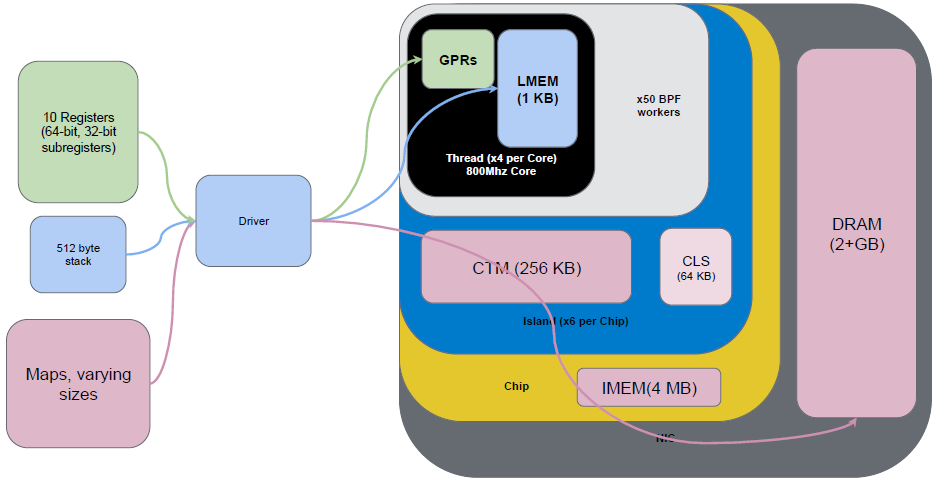
\includegraphics[width=0.4\textwidth]{figures/ebpf_offload.png}
    \caption{Netronome's solution to SmartNIC eBPF offload \cite{beckett:2018:ebpf-xdp}.}
    \label{fig:ebpf-offload}
\end{figure}

Very recently, however, researchers addressing the problem of reducing jitter of very small applications running in data centers, called lambda-applications, have proposed an approach we can be inspired by. The authors of \cite{tork:2020:lynx} proposed that smartNICs, instead of running lambda applications in their cores as proposed in \cite{choi:2019:lambda-nic}, forward data received from the network to be processed by a GPU via Peer-to-Peer (P2P) PCIe communication, without the need for operating system manipulation, as illustrated in Figure-\ref{fig:lynx}. The results are then sent back to the smartNIC and forwarded to the network.

\begin{figure}[ht]
    \centering
    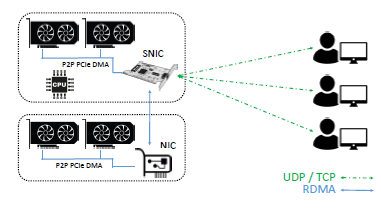
\includegraphics[width=0.4\textwidth]{figures/linx.png}
    \caption{SmartNIC forwarding data straight to GPU for processing acceleration \cite{tork:2020:lynx}.}
    \label{fig:lynx}
\end{figure}

\section{Hypothesis}
Our hypothesis for this research is that we can significantly reduce the time CPU cores spend filtering packets by offloading to an integrated solution between a NIC and an eBPF accelerator.

\section{Project Proposal}
Inspired by the works in Section \ref{sec:rel-works}, we propose a research for the development of a high level scallable micro architecture, as \cite{ankit2019puma}, able to run multiple eBPF programs in parallel and to communicate with a network card to offload the packet filer processing from the CPUs. The network card should be able to send ingress packets to eBPF offload cards via P2P before they reach the Operating System, integrating to its SR-IOV implementation for enhanced support for virtualization.

\section{Questions to be answered}
Before proceeding with the research, we need to answer the following questions:
\begin{itemize}
    \item How much of CPU time dedicated to packet filtering can we save with such an approach?
    \item Which measures apply if we implement the final solution in software to assess its efficacy?
\end{itemize}

\bibliographystyle{IEEEtran}
\bibliography{library}

\end{document}
